\documentclass[12pt]{article}

\usepackage{times}
\usepackage{textcomp}
\usepackage{listings}
\usepackage{fullpage}
\usepackage{color}
\usepackage{hyperref} 
\usepackage{pst-tree} 
\usepackage{verbatim} 
\usepackage{graphicx}
\usepackage{amsmath,amsfonts,amssymb,amsthm}
\graphicspath{{./}}
\usepackage{courier}

\lstset{language=C, keywordstyle={\bfseries \color{red}}, basicstyle=\footnotesize\ttfamily}

\author{Clement Tsang}

\begin{document}

\begin{center}
\Large\textbf{CS 241, Lecture 22: Heap Management and Loaders}
\end{center}

\section{Heap}
\begin{itemize}
    \item The \textbf{Binary Buddy System}: we start with, say, 512 bytes of heap memory.  Suppose we try to allocate 19 bytes.  We need one more for bookkeeping, so we allocate 20 bytes.  This fits in a block size of $2^5 = 32$ bytes.  So we spolit our memory until we find such a block, and reserve the entire block.
    \item So our block starts like $[512]$ and ends with $[\textbf{32}|32|64|128|256]$ (bold is reserved).  
    \item Now let's next request 63 bytes (which requires 64 bytes of space).  This gives us something along the lines of $[\textbf{32}|32|\textbf{64}|128|256]$ 
    \item Now let's request 40 bytes --- as we know, this becomes 41 bytes.  We need a 64 byte block we don't have, so we split the 128 block and get: $[\textbf{32}|32|\textbf{64}|\textbf{64}|64|256]$ 
    \item Now let's free the 63 block.  We get: $[\textbf{32}|32|64|\textbf{64}|64|256]$ 
    \item Now free the 19 byte block, giving us $[32|32|64|\textbf{64}|64|256]$.  We can collapse 32 and it's neighbouring buddy, giving us $[64|64|\textbf{64}|64|256]$, from which we can then collapse into $[128|\textbf{64}|64|256]$.
    \item Now finally, free the 40 byte block, giving us $[128|64|64|256]$, which we repeatedly collapse to get our original $[256]$ block of memory.
    \item Some languages are nice, and they provide automatic memory management, like Java.  How is this done?
    \item One technique is \textbf{reference counting}.  The idea is that for each heap block, keep track of the number of pointers that point to it.
    \item We must watch every pointer and update reference counts each time a pointer is reassigned.
    \item If a block's reference count reaches 0, reclaim it.
    \item If a block points to another block and vice versa (and nothing points to the cluster), then the cluster is unreachable and should be cleaned.
    \item Another technique is \textbf{marking and sweeping}.  Here, we scan the entire stack and global variables, and search for pointers.  We mark the heap blocks that have pointers to them.  We then scan the heap and reclaim any blocks that aren't marked.  
    \item Essentially, this is a graph traversal problem.
    \item A third technique is \textbf{copying the collector}.  The idea is to split the heap into two halves, say, $H_1$ and $H_2$.  Allocate memory in $H_1$, and when it is full or we cannot find enough memory, copy $H_1$ into $H_2$.  
    \item After the copy, $H_2$ has all the memory stored contiguously.  Then, from now on, allocate to $H_2$ (in essence, flip the roles of $H_1$ and $H_2$).
    \item This leaves no fragmentation, and \lstinline[mathescape]{new} and \lstinline[mathescape]{delete} are very quick --- but we can only use half the heap at a time!
    \item A more common variant is to split the heap into 3 or 4 regions, and reserve one region for the copy step instead.
\end{itemize}

\section{Loaders}
\begin{itemize}
    \item Let's write the dumbest but techinically correct operating system:
\begin{lstlisting}[mathescape, numbers=none, breaklines=true]
repeat:
    P <- next program to run
    copy P into memory at 0x0
    jalr $\$$0
    beq $\$$0, $\$$0, repeat
\end{lstlisting}
        Note that this is how \lstinline[mathescape]{mips.twoints} and \lstinline[mathescape]{mips.array} work.
    \item The operating system is a program that needs to be in memory --- where should it be?
    \item We let the loader deside instead of choosing different addresses at assembly time, which may lead to collisions.
    \item So the loader's job is to:
        \begin{itemize}
            \item Take a program $P$ as input
            \item Find a location $\alpha$ in memory for $P$
            \item Copy $P$ to memory, starting at $\alpha$
            \item Return $\alpha$ to the OS
        \end{itemize}
    \item Introducing our OS, version 2.0:
\begin{lstlisting}[mathescape, numbers=none, breaklines=true]
repeat:
    P <- next program to run
    $\$$3 <- loader(P)
    jalr $\$$3
    beq $\$$0, $\$$0, repeat
\end{lstlisting}
    \item Our input is machine code in the form of words, from $w_1$ to $w_k$.  Note that $n = k + stack_space$, which is how much space we keep for the stack (if the name wasn't self-explanatory)
    \item This gives us code like:
\begin{lstlisting}[mathescape, numbers=none, breaklines=true]
for i from i to k:
    MEM[alpha + 4 * i] = w_i
$\$$30 <- alpha + 4 * n
return alpha
\end{lstlisting}
    Unfortunately, there are some issues with this approach: labels may be resolved to incorrect addresses!
    \item So to solve this, we might do something like:
\begin{lstlisting}[mathescape, numbers=none, breaklines=true]
.word id <- need to add alpha to id
.word constant <- do not reallocate!
branching commands etc. <- do not reallocate!
\end{lstlisting}
    \item But recall that we need to translate assembly code into machine code.  So given \lstinline[mathescape]{0x00000018}, is this a \lstinline[mathescape]{.word constant} or a \lstinline[mathescape]{.word id}?  We don't know!
    \item Introducing OS 3.0:
\begin{lstlisting}[mathescape, numbers=none, breaklines=true]
repeat:
    P <- next program to run
    $\$$3 <- load_and_relocate(P)  ;note that we haven't determined how to relocate
    jalr $\$$3
    beq $\$$0, $\$$0, repeat
\end{lstlisting}
    \item Usually, the output of assemblers is not pure machine code, it's object code.
    \item We see this in our MERL(MIPS Executable Relocatable Linkable) files.
    \item In this file, we need the code, location of \lstinline[mathescape]{.word id}, and some auxiliary information.
    \item So for example:
\begin{lstlisting}[mathescape, numbers=none, breaklines=true]
beq $\$$0, $\$$0, 2
.word endfile ;file length
.word endcode ;code + header
;Insert MIPS Assembly here
.word 0x4 ;constant no relocation
.word 0x8 ;constant no relocation
.word A ;needs relocation
B: jr $\$$31
A: beq $\$$0, $\$$, B ;no relocation
endcode:    ;MERL symbol table
.word 0x1   ;format code 1 means relocate
.word 0x14  ;location of A
endfile:
\end{lstlisting}
    \item Note this requires two passes - the first pass records the size of the file, starts counting address at 0x0c instead of 0x0, and record the location of \lstinline[mathescape]{.word id} instructions.  The second pass outputs the header, MIPS machine code, and relocation table.
    \item Note that even with this, it is possible to write code that only works at address 0.  For example:
\begin{lstlisting}[mathescape, numbers=none, breaklines=true]
lis $\$$2
.word 12
jr $\$$2
jr $\$$31
\end{lstlisting}
    We should never encode address as anything other than labels, so that your loader can update the references --- that is, \textbf{NEVER hardcode addresses}!
    \item our loader relocation algorithm is as follows:
\begin{lstlisting}[mathescape, numbers=none, breaklines=true]
read_line() // skip cookie
endMod <-- read_line() // end of MERL file
codeLen <- read_line - 12 // no header in codeLen
alpha <- findFreeRAM(codeLen)
for (int i = 0; i < codeLen; ++i) 
    MEM[alpha + i] <- read_line()
i <- codeLen + 12 // start of relocation table
while (i < endMod)
    format <- read_line()
    if (Format == 1)
        rel <- read_line()
        // go forward by alpha and back by header len
        // alpha + rel - 12 since we don't load header
        MEM[alpha + rel - 12] += alpha - 12
    else
        ERROR
    i += 8
\end{lstlisting}
    \item How do we resolve situations where we have labels in different files?
    \item We could \lstinline[mathescape]{cat} all such files together, but why should we reassemble these files more than once?
    \item A better solution is the assemble the files first, \textbf{then} cat$\cdot$ right?
    \item But remember only one piece can be at \lstinline[mathescape]{0x0} at a time --- so those assembled files need to be MERL files, and not just MIPS files.
    \item Note that concatenating two MERL files does not give a valid MERL file!
    \item More doom!  We haven't really resolved the issue with labels in different files.  
    \item We need to modify our assembler --- when we encounter a \lstinline[mathescape]{.word} where the label is not in the file, we need to print a placeholder, \lstinline[mathescape]{0x0} in our case, and indicate that we cannot run this program until our value of the \lstinline[mathescape]{id} is given.
    \item For example, consider the following two \lstinline[mathescape]{.asm} files:
\begin{lstlisting}[mathescape, numbers=none, breaklines=true]
a.asm:

lis $\$$3
.word label

===

b.asm:

label: sw $\$$5, -4($\$$30)
\end{lstlisting}
    where we cannot run \lstinline[mathescape]{a.asm} without linking with \lstinline[mathescape]{b.asm} 
    \item We need to extend our MERL file so that it can notify us when we need to assemble with multiple files.
    \item Now let's consider another (related) thing --- error checking.  Let's say we had a typo:
\begin{lstlisting}[mathescape, numbers=none, breaklines=true]
lis $\$$3
.word banana
bananas:
\end{lstlisting}
    \item Did we make a mistake?  How do we recognize this error?  Without any changes, our assembler might believe this label, \lstinline[mathescape]{banana}, exists elsewhere and load this with a placeholder --- this might not be desired!
    \item How do we tell our assembler what is an error and what is intentional?
    \item \lstinline[mathescape]{.import id} is the command which asks for which \lstinline[mathescape]{id} we should be linking in.
    \item This does not assemble to a word of MIPS.
    \item Errors will occur if the label \lstinline[mathescape]{id} is not in the current file and there is no \lstinline[mathescape]{.import id} in the file.
    \item We need to add entries in the MERL symbol table, and include format code \lstinline[mathescape]{0x11} for External Symbol Reference(ESR).
    \item What needs to be in an ESR entry?
        \begin{itemize}
            \item Where the symbol is being used
            \item The name of said symbol
        \end{itemize}
       For example:
\begin{lstlisting}[mathescape, numbers=none, breaklines=true]
0x11 ;format code
;location used
;length of the name in symbol (n)
;1st ASCII char of the name of symbol
;2nd ASCII char of the name of symbol
...
;nth ASCII char of the name of symbol
\end{lstlisting}
    \item Another fun problem --- what if lables are duplicated.  We wouldn't want to export a label in this situation --- this is why we have the \lstinline[mathescape]{.export} directive.
    \item \lstinline[mathescape]{.export label} makes \lstinline[mathescape]{label} avaliable for linking with other files.  Like import, it doesn't translate to a word in MIPS, but rather tell the assembler to make an entry in the MERL symbol table.
    \item The assembler makes an ESD, or an External Symbol Definition, for these words, following the format:
\begin{lstlisting}[mathescape, numbers=none, breaklines=true]
0x05 ;format code
;address the symbol represents
;length of name of symbol(n)
;1st ASCII char
...
;nth ASCII char
\end{lstlisting}
    \item Now, our MERL file contains the code, the address that needs relocating, as well as the addresses and names of every ESR and ESD.  Our linker is complete.
    \item Linker algorithm:\\
        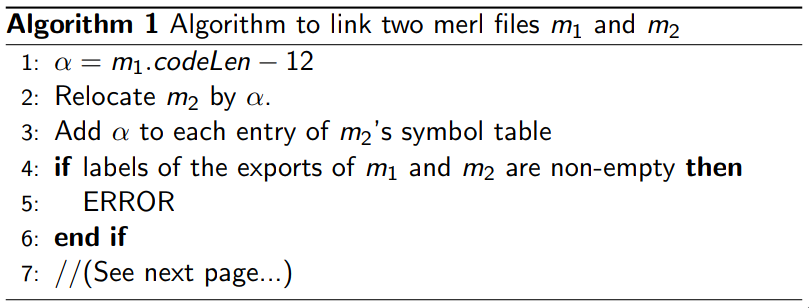
\includegraphics[scale=0.5]{link_1.png}\\
        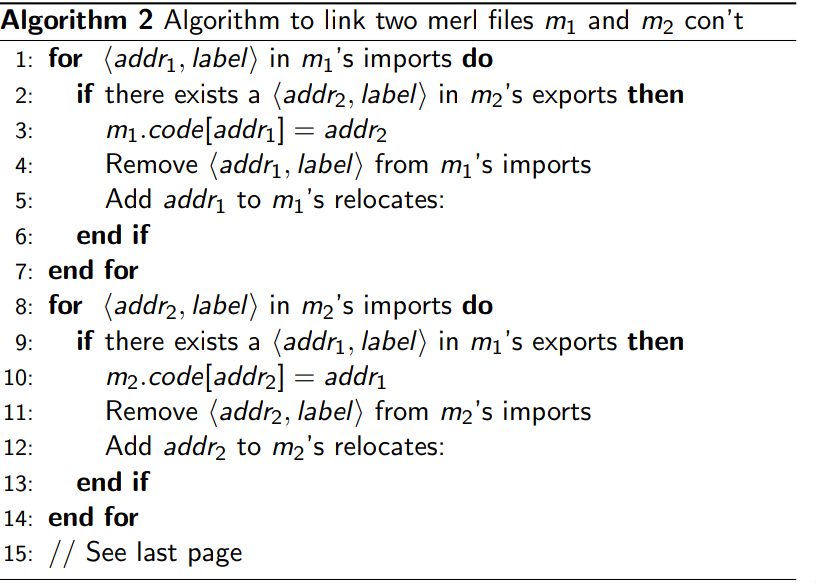
\includegraphics[scale=0.5]{link_2.png}\\
        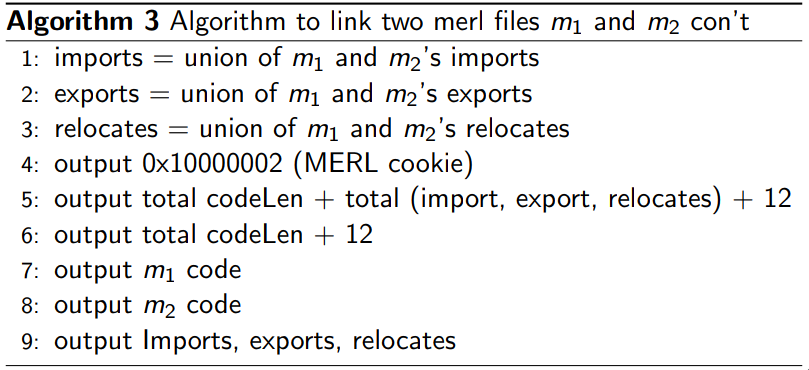
\includegraphics[scale=0.5]{link_3.png}
\end{itemize}

\end{document}

